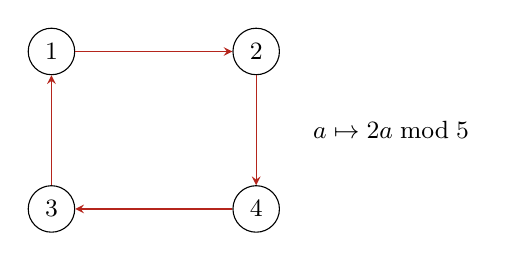
\begin{tikzpicture}[>=stealth,font=\small]
\foreach \x/\y/\v in {0/1/1,2.6/1/2,2.6/-1/4,0/-1/3}{\node[draw,circle] (n\v) at (\x,\y) {$\v$};}
\draw[->,BrickRed] (n1)--(n2);
\draw[->,BrickRed] (n2)--(n4);
\draw[->,BrickRed] (n4)--(n3);
\draw[->,BrickRed] (n3)--(n1);
\node[right] at (3.2,0) {$a\mapsto2a\bmod5$};
\end{tikzpicture}
